\documentclass[../main.tex]{subfiles}
\graphicspath{
    {"../img/"}
    {"img/"}
}


\begin{document}

    \subsection{Zabawki działające dzięki wnioskom z Tw. wyżej - funkcje uwikłane}

\[
    x+y=1 \quad\text{(a)}
.\]
\[
    x^2+y^2=1 \quad\text{(b)}
.\]
\[
    H(x,y) = \sin x e^{xy}+ \tg y - x = 0
.\]


\vspace{2cm}

\begin{figure}
    \centering
    \includegraphics[width=0.8\textwidth]{fig_7}
    \caption{(a)}
\end{figure}
\begin{figure}
    \centering
    \includegraphics[width=0.8\textwidth]{fig_8}
    \caption{(b)}
\end{figure}
\begin{figure}
    \centering
    \includegraphics[width=0.6\textwidth]{fig_9}
    \caption{(c)}
\end{figure}


\vspace{1cm}

\begin{przyklad}
    Równanie gazowe
\end{przyklad}
    \[
        H(p,V,T) = 0, H: \mathbb{R}^{3} \to \mathbb{R}^{1}
    .\]
    \[
        p(V,T) = 0, \mathbb{R}^{2}\to\mathbb{R}^{1}
    .\]
    \[
        V(p,T) = 0, \mathbb{R}^{2}\to\mathbb{R}^{1}
    .\]
    \[
        T(p,V) = 0, \mathbb{R}^{2}\to\mathbb{R}^{1}
    .\]
    \textit{istnienie przedziałów, w których funkcja uwikłana zadaje inne funkcje}

    \begin{przyklad}
        \[
            H(x,y): U\subset\mathbb{R}^2\to\mathbb{R}^1
        .\]
    \end{przyklad}
    \begin{pytanie}
        Czy istnieje $y(x): H(x,y(x)) = 0$, dla  $x\in V$?
    \end{pytanie}
    \[
        \frac{dH}{dx}(x,y(x)) = \frac{d}{dx}(H(x,y)\circ g(x))
    .\]
    \[
        H' = \left[   \frac{\partial H}{\partial x} ,\frac{\partial H}{\partial y} \right]
    .\]
    \[
        g(x): \mathbb{R}^{1}\to\mathbb{R}^{2}, g(x) = \begin{bmatrix}
        x\\
    y(x)\\\end{bmatrix}, g'(x) = \begin{bmatrix}
1\\
y'(x)\\\end{bmatrix}
    .\]
    \[
        H'(x,y) g'(x) = 0 \implies \frac{\partial H}{\partial x} + \frac{\partial H}{\partial y} \frac{\partial y}{\partial x} =0 \implies \frac{\partial y}{\partial x} = - \frac{\frac{\partial H}{\partial x} }{\frac{\partial H}{\partial y} }
    .\]
    Więc
    \[
        \frac{\partial y}{\partial x}  = \frac{-\cos y + ye^{xy} -1}{xe^y + \frac{1}{\cos^2 y }}
    .\]
    \begin{przyklad}

    \end{przyklad}
    \[
        H(x_{1},x_{2},x_{3},x_{4},x_{5}) = \begin{bmatrix}   2e^{x_1}+x_{2}x_{3} - 4x_{3}+3\\
            x^2 \cos x_{1} - 6x_{1}+2x_{3}-x_{5}, H:\mathbb{R}^{5}\to\mathbb{R}^{3}
\end{bmatrix}
    .\]
    \[
        H(x_{1},\dots,x_{5}) = 0 \text{ może zadać funkcję }g:\mathbb{R}^{3}\to\mathbb{R}^{2}
    .\]
    \[
        x_{4}(x_{1},x_{2},x_{3}),x_{5}(x_{1},x_{2},x_{3})
    .\]
    \[
        g(x_{1},g_{2},g_{3}) = \begin{bmatrix}
        g_1(x_{1},x_{2},x_{3})\\
    g_2(x_{1},x_{2},x_{3}\\
\end{bmatrix}
    .\]

    \begin{obserwacja}
        $H(0,1,3,2,7) = 0$
    \end{obserwacja}

    \[
        H: \mathbb{R}^{5}\to\mathbb{R}^{2}, H(x_{1},x_{2},y_{1},y_{2},y_{3}) = 0
    .\]
    \[
        H(x_{1},x_{2},y_{1},y_{2},y_{3}) = \begin{bmatrix}
        H_1(x_{1},x_{2},y_{1},y_{2},y_{3})\\
    H_2(x_1,x_2,y_1,y_2,y_2)\\\end{bmatrix}
    .\]
    \begin{pytanie}
        Czy $H(x_1,x_2,y_1,y_2,y_3) = 0$ zadaje nam \[
            g_1(y_1,y_2,y_3)\\
        .\]
        \[
            g_2(y_1,y_2,y_3)?
        \]
    \end{pytanie}
    czyli $g(y_1,y_2,y_3) = \begin{bmatrix}
    g_1(y_1,y_2,y_3)\\
g_2(y_1,y_2,y_3)\\\end{bmatrix}, g:\mathbb{R}^{3}\to\mathbb{R}^{2}$

\[
    H_1(g_1(y_1,y_2,y_3),g_2(y_1,y_2,y_3),y_1,y_2,y_3) = 0
.\]
\[
    H_2(g_1(y_1,y_2,y_3),g_2(y_1,y_2,y_3),y_1,y_2,y_3) = 0
.\]
Szukamy $g'$.
 \[
g' = \begin{bmatrix}
\frac{\partial g_1}{\partial y_1} & \frac{\partial g_1}{\partial y_2} &\frac{\partial g_1}{\partial y_3} \\
\frac{\partial g_2}{\partial y_1} &\frac{\partial g_2}{\partial y_2} &\frac{\partial g_3}{\partial y_3} \\\end{bmatrix}
.\]

\[
\frac{\partial H_1}{\partial x_1} \frac{\partial g_1}{\partial y_2} +\frac{\partial H_1}{\partial x_2} \frac{\partial g_2}{\partial y_1} +\frac{\partial H_1}{\partial y_1} = 0
.\]

\[
\frac{\partial H_1}{\partial x_1} \frac{\partial g_1}{\partial y_3} +\frac{\partial H_1}{\partial x_2} \frac{\partial g_2}{\partial y_1} +\frac{\partial H_1}{\partial y_1} = 0
.\]

\[
\frac{\partial H_1}{\partial x_1} \frac{\partial g_1}{\partial y_3} +\frac{\partial H_1}{\partial x_2} \frac{\partial g_2}{\partial y_3} +\frac{\partial H_1}{\partial y_3} = 0
.\]

\[
\frac{\partial H_2}{\partial x_1} \frac{\partial g_1}{\partial y_1} +\frac{\partial H_2}{\partial x_2} \frac{\partial g_2}{\partial y_1} +\frac{\partial H_2}{\partial y_1} = 0
.\]

\[
\frac{\partial H_2}{\partial x_1} \frac{\partial g_1}{\partial y_2} +\frac{\partial H_2}{\partial x_2} \frac{\partial g_2}{\partial y_2} +\frac{\partial H_2}{\partial y_2} = 0
.\]

\[
\frac{\partial H_2}{\partial x_1} \frac{\partial g_1}{\partial y_3} +\frac{\partial H_2}{\partial x_2} \frac{\partial g_2}{\partial y_3} +\frac{\partial H_2}{\partial y_3} = 0
.\]
napięcie rośnie (6 równań oho)

\[
    \underset{H_x'}{\begin{bmatrix}
\frac{\partial H_1}{\partial x_1} &\frac{\partial H_1}{\partial x)2} \\
\frac{\partial H_2}{\partial x_1} &\frac{\partial H_2}{\partial x_2} \end{bmatrix}}
\underset{g'}{\begin{bmatrix}
\frac{\partial g_1}{\partial y_1} &\frac{\partial g_1}{\partial y_2} &\frac{\partial g_1}{\partial y_3} \\
\frac{\partial g_2}{\partial y_1} &\frac{\partial g_2}{\partial y_2} &\frac{\partial g_2}{\partial y_3} \end{bmatrix}}
= -
\underset{H_y'}{\begin{bmatrix}
\frac{\partial H_1}{\partial y_1} &\frac{\partial H_1}{\partial y_2} &\frac{\partial H_1}{\partial y_3} \\
\frac{\partial H_2}{\partial y_1} &\frac{\partial H_2}{\partial y_2} &\frac{\partial H_2}{\partial p_3} \end{bmatrix}}
.\]

\[
    H_x' g' = -H_y' \implies g' = -(H_x')^{-1}H_y'
.\]

\pagebreak
\begin{tw}
    (o funkcji uwikłanej)\\
    Niech
    \begin{align*}
        &H:E\subset\mathbb{R}^{n+m}\to\mathbb{R}^{m},\\
        &H\in\mathcal{C}^{1} \text{ na } E. (x_0,y_0)\in E, \\
        &H(x_0,y_0)=0, \\
        &(x_0,y_0) = (x_0^1,\ldots,x_0^n,y_0^1,\ldots,y_0^m), \\
        &H \text{ - odwracalna}.
    .\end{align*}
    Wówczas istnieje  $U\subset E$ takie, że $(x_0,y_0)\in U, \underset{W\subset \mathbb{R}^{n}}{\exists} $, że
    \[
        x_0\in W, \underset{x\in W}{\forall} \underset{y}{\exists !} H(x,y) = 0, (x,y) \in U.
    \]
    Jeżeli $y= \varphi(x)$, to
    \[
        \varphi:\mathbb{R}^{n}\to\mathbb{R}^{m} \text{ i } \varphi\in \mathcal{C}^{1}(W),
    \]
    \[
         \varphi'(x) = -(H_y')^{-1}H_x'
     .\]
\end{tw}

\begin{proof}
    Oznaczenia:
    \[
        H(x^1,\ldots,x^n,y^1,\ldots,y^m) = \begin{bmatrix}
        H^1(x^1,\ldots,x^n,y^1,\ldots,y^m)\\
        \vdots\\
        H^2(x^1,\ldots,x^n,y^1,\ldots,y^m)\\
    \end{bmatrix}
    .\]
    \[
    H_y' = \begin{bmatrix}
    \frac{\partial H^1}{\partial y^1} &\ldots&\frac{\partial H^1}{\partial y^n} \\
    \vdots&\ddots&\vdots\\
\frac{\partial H^m}{\partial y^1} &\ldots&\frac{\partial H^m}{\partial y^n} \end{bmatrix},
    H_x' = \begin{bmatrix}
    \frac{\partial H^1}{\partial x^1} &\ldots&\frac{\partial H^1}{\partial x^n} \\
    \vdots&\ddots&\vdots\\
\frac{\partial H^m}{\partial x^1} &\ldots&\frac{\partial H^m}{\partial x^n} \end{bmatrix}
    .\]
    Wprowadźmy funkcję $F:\mathbb{R}^{n+m}\to\mathbb{R}^{n+m}$
    \[
        F(x^1,\ldots,x^n,y^1,\ldots,y^m) = \begin{bmatrix}
        x^1\\
    x^2\\
\vdots\\
x^n\\
H^1(x^1,\ldots,x^n,y^1,\ldots,y^m)\\
\vdots\\
H^m(x^1,\ldots,x^n,y^1,\ldots,y^m)\\
\end{bmatrix}
    .\]
    Jakie własności ma $F$?
    \[
        F(x_0,y_0) = \begin{bmatrix}
        x_0\\
        y_0\end{bmatrix} = \begin{bmatrix}
        x_0\\
        0\end{bmatrix}
    .\]
    Ale \[
    F' = \begin{bmatrix}
        1&&&&0\\
         &\ddots&&&\\
         &&1&&\\
         &&&&\\
         &H_x'&&&H_y'
    \end{bmatrix}, \det F' = \det H_y'
    .\]
    \begin{figure}[h]
        \centering
        \includegraphics[width=0.7\textwidth]{fig_10}
        \caption{}
        \label{fig:}
    \end{figure}

    Jeżeli $H_y'(x_0,y_0)$ - odwracalna, to $F'(x_0,y_0)$ - też.
    Oznacza to (na podstawie tw. o lokalnej odwracalności), że
    \[
        \underset{U\subset\mathbb{R}^{n+m}}{\exists},
        (x_0,y_0)\in U, \underset{V\subset\mathbb{R}^{n+m}}{\exists} ,(x_0,0)\in V
    .,\] że $F$ jest bijekcją między $U$ i $V$ oraz $\exists F^{-1}:V\to U, F^{-1}$ - różniczkowalna taka, że
     \[
         F^{-1}(x,\alpha) = (a(x,\alpha),b(x,\alpha)), x,\alpha\in V
     .,\] gdzie $a(x,\alpha): \mathbb{R}^{m+n}\to\mathbb{R}^n,\quad b(x,\alpha):\mathbb{R}^{m+n}\to\mathbb{R}^m  $

    Dla $(x',y')\in \mathcal{V},$
    \[
        F^{-1}(x',y') = (a(x',y'),b(x',y'))
    .\]
    Wiemy, że $a: \mathbb{R}^{n+m}\to\mathbb{R}^{n}$ i $b: \mathbb{R}^{n+m}\to\mathbb{R}^m$ istnieją i są różniczkowalne, bo $F^{-1}$ istnieje. Co jeszcze wiemy o funkcjach $a$ i $b$?\\
    Wiemy że  \[
        (x',y') = F(F^{-1}(x',y') = F(\underbrace{a(x',y')}_{n} , \underbrace{b(x',y')}_{m})
    .\]
    Oznacza to, że
    \[
        a(x',y') = x'
    .\]
    Czyli $a(x',y')$ jest identycznością, czyli:
    \[
        (x',y') = F(x',b(x',y')) \implies x'=x \implies (x,y') = F(x,b(x,y'))
    .\]
    Czyli jeżeli $y=b(x,0)$, to wtedy
    \[
        F(x,y) = (x,0)\text{, czyli } (x,H(x,y)) = (x,0)
    .\]
    Czyli dla $y = (x,0)$ otrzymujemy, że
    \[
        H(x,y)=0
    .\]
    Jeżeli oznaczymy $b(x,0) \overset{\text{ozn}}{=} \varphi(x)$, to znaczy, że znaleźliśmy funkcję $\varphi(x), \varphi:\mathbb{R}^n\to\mathbb{R}^m$ taką, że \[
        H(x,\varphi(x))=0
    .\]

\end{proof}

\begin{figure}[h]
    \centering
    \includegraphics[width=0.8\textwidth]{fig_11}
    \caption{}
    \label{fig:}
\end{figure}



\end{document}

